\section{Archetypes}
\note{
    \begin{itemize}
        \item TODO: Intuition of why and how we created these
    \end{itemize}
}

\begin{frame}{3 Archetypes}
    \newlength{\onethird}
    \setlength{\onethird}{0.315\textwidth}
    \vspace{.2cm}
    \begin{minipage}[t]{\onethird}
        \centering
        \textbf{Autocratic Collector\vphantom{j}}\\
        \vspace{.6cm}
        \scalebox{0.8}{
        \begin{tikzpicture}[auto]
            \pgfdeclarelayer{background}
            \pgfsetlayers{background,main}
            \node[block] (input) {Private external\\entropy source};
            \node[block, below=1cm of input] (computation) {Computation\\$f(I_t)$};
            \node[block, below=1cm of computation] (users) {Users};
            \draw[arrow] (input) -- node (inp) {$I_t$} (computation);
            \draw[arrow] (computation) -- node {$O_t$} (users);
            \begin{pgfonlayer}{background}
                %\node[block] (beacon) [container, fit={(input) (computation)}] {};
            \end{pgfonlayer}
        \end{tikzpicture}
        }
    \end{minipage}
    ~~\begin{minipage}[t]{\onethird}
        \centering
        \textbf{Special MPC}\\
        \vspace{.6cm}
        \scalebox{0.8}{
        \begin{tikzpicture}[auto]
            \pgfdeclarelayer{background}
            \pgfsetlayers{background,main}
            \node[block] (input) {Each user's input};
            \node[block, text width=9em, below=1cm of input] (computation) {Partial computation\\$f'(I'_t)$};
            \node[block, below=1cm of computation] (users) {Users};
            \draw[arrow] (input) -- node (inp) {$I_{u,t}$} (computation);
            \draw[arrow] (computation) -- node {$O_t$} (users);
            \draw[arrow] (computation.south) to [out=250, in=250, looseness=2] node[shift={(-7mm,3mm)}] (rprime) {$O'_t$} ([shift={(-10mm,0mm)}]computation.south);
            \begin{pgfonlayer}{background}
                %\node[block] (beacon) [container, fill=GoogleLightBlue!40, draw=GoogleLightBlue, fit={(input) (computation) ([shift={(0mm,3mm)}]rprime.south west)}] {};
            \end{pgfonlayer}
        \end{tikzpicture}
        }
    \end{minipage}
    ~~\begin{minipage}[t]{\onethird}
        \centering
        \textbf{Transparent Authority}\\
        \vspace{.6cm}
        \scalebox{0.8}{
        \begin{tikzpicture}[auto]
            \pgfdeclarelayer{background}
            \pgfsetlayers{background,main}
            \node[block] (input) {Verifiable input};
            \node[block, below=1cm of input] (computation) {Computation\\$f(I_t)$};
            \node[block, below=1cm of computation] (users) {Users};
            \draw[arrow] (input) -- node (inp) {$I_t$} (computation);
            \draw[arrow] (computation) -- node {$O_t$} (users);
            \begin{pgfonlayer}{background}
                %\node[block] (beacon) [container, fill=GoogleBlueGrey!40, draw=GoogleBlueGrey, fit={(computation)}] {};
            \end{pgfonlayer}
        \end{tikzpicture}
        }
    \end{minipage}
\end{frame}
\note{
    \begin{itemize}

        \item For all types, the output is the same. Users can use the output from all types for all the use cases.
    \end{itemize}
}

\begin{frame}{Autocratic Collector: The NIST Beacon}
    \begin{columns}
        \begin{column}{0.7\textwidth}
						\vspace{.5cm}
            \begin{itemize}
                \item \textsc{\textbf{Input:}} Output from a photon splitter
								\item \textsc{\textbf{Computation:}} ---
                \item \textsc{\textbf{Output:}} 512 bits every 60 seconds
								%\begin{itemize}
								%  \item The output at January 17, 15:11 (UTC)\\
								%	      \texttt{\scriptsize 67AE66B6E1812F4D32064B834A5E1AD5\\1424DCBC18DF8A9AAE2B8B7FA409002E\\9E314045F6E595A8EEBBB027CFBB4D8B\\BA64007F6EAE3EC92051ADD8391DA2B9\\}
								%\end{itemize}
								
            \end{itemize}
						\vspace{.7cm}\centering
						{%
							\setlength{\fboxsep}{0pt}%
							\setlength{\fboxrule}{.75pt}%
							\fbox{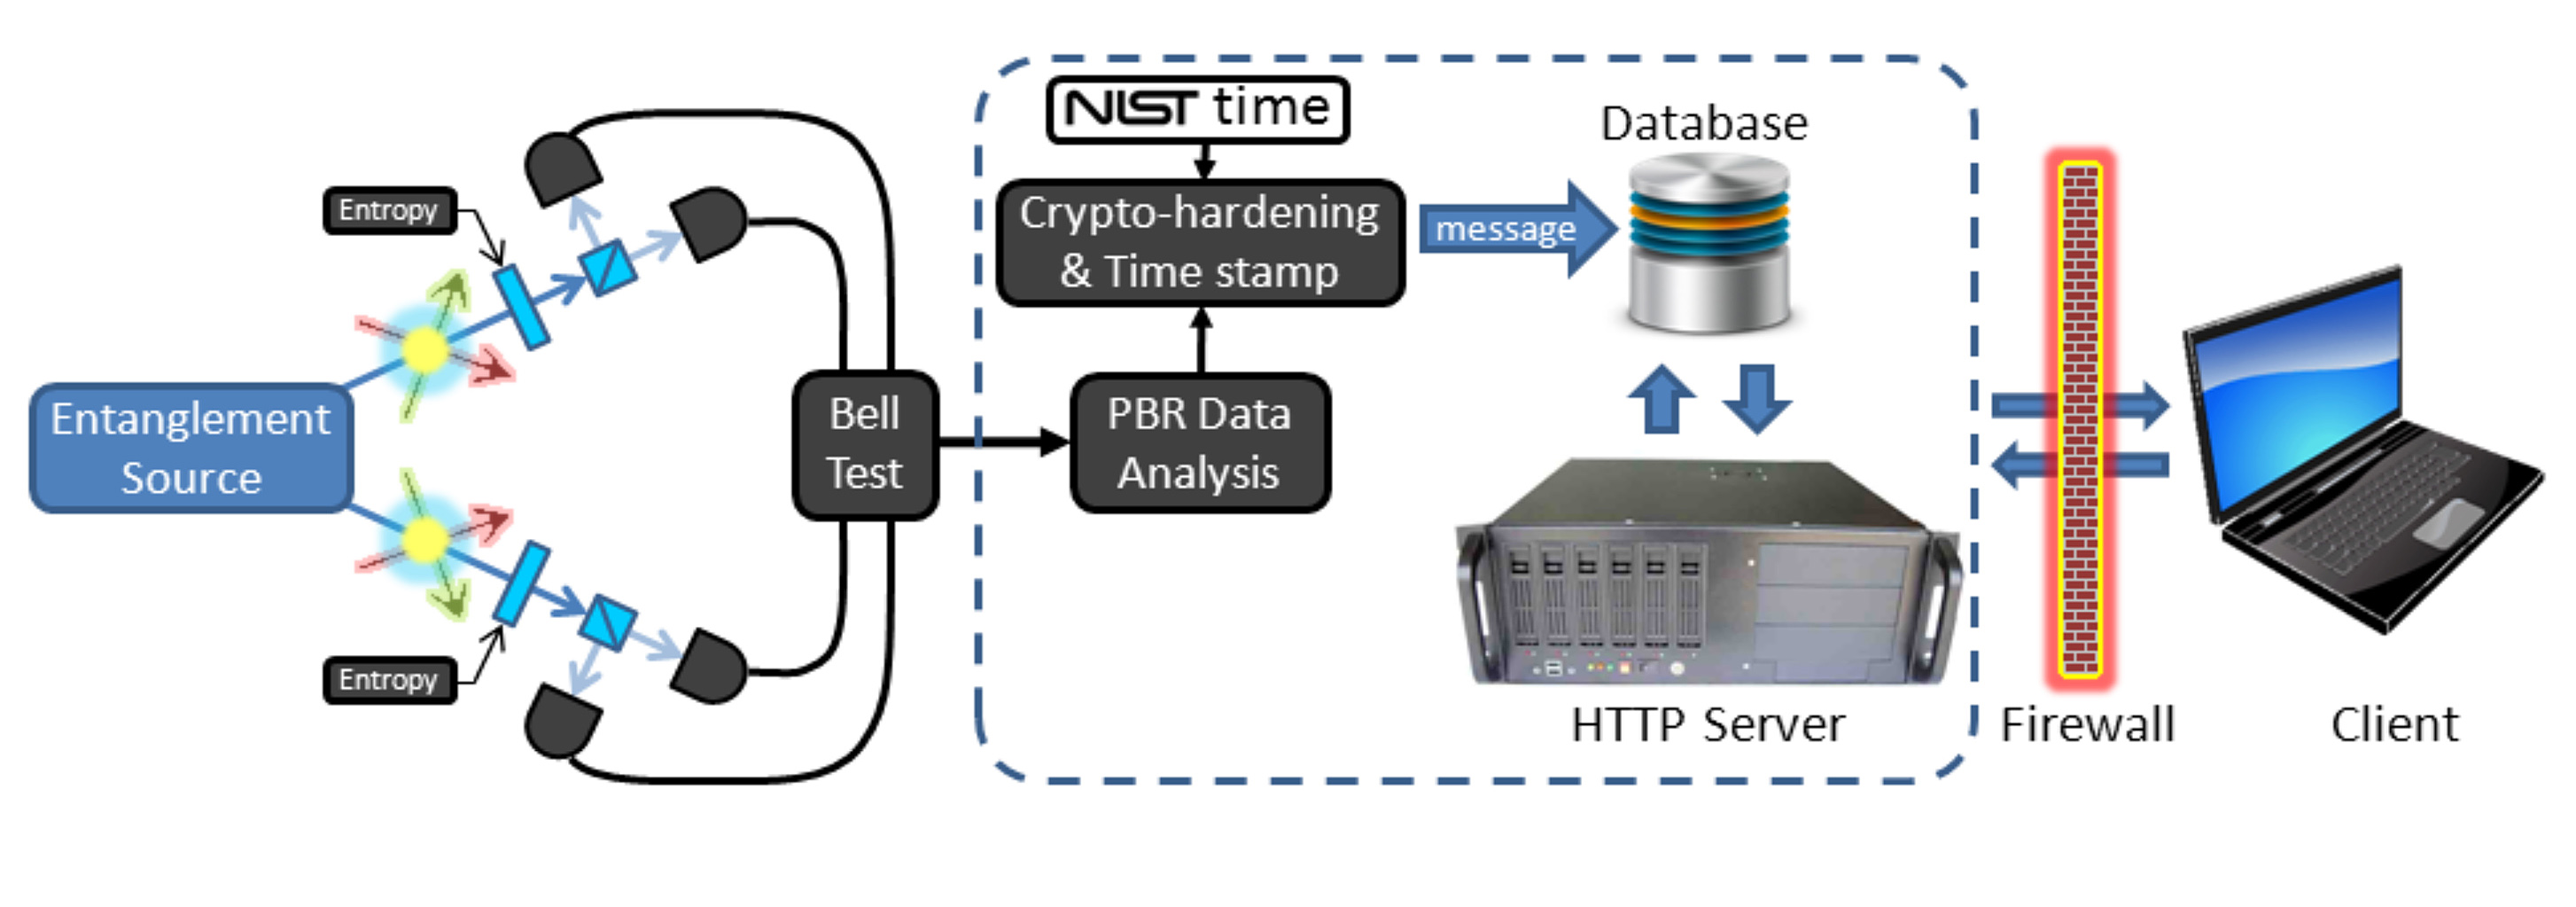
\includegraphics[width=.95\textwidth]{figures/nist.jpg}}\\
							\tiny
							\vspace{-1.5em}Image source: NIST%
						}%
        \end{column}
        \begin{column}{0.3\textwidth}
            \begin{center}
                \scalebox{0.85}{
                \begin{tikzpicture}[auto]
                    \pgfdeclarelayer{background}
                    \pgfsetlayers{background,main}
                    \node[block] (input) {Private external\\entropy source};
                    \node[block, below=.7cm of input] (computation) {Computation\\$f(I_t)$};
                    \node[block, below=1.2cm of computation] (users) {Users};
                    \draw[arrow] (input) -- node (inp) {$I_t$} (computation);
                    \draw[arrow] (computation) -- node[yshift=-1mm] {$O_t$} (users);
                    \begin{pgfonlayer}{background}
                        \node[block] (beacon) [container, fit={(input) (computation)}] {};
                    \end{pgfonlayer}
                \end{tikzpicture}
                }
             \end{center}
        \end{column}
    \end{columns}

\end{frame}
\note{
    \begin{itemize}
        \item We don't know if it has been tampered with. There is no way of knowing for sure.
        \item What attack types are most particular for this type?

    \end{itemize}

}

\begin{frame}{Special MPC: RandHerd}
    \begin{columns}
        \begin{column}{0.7\textwidth}
            \begin{itemize}
                \item \textsc{\textbf{Hierarchy:}}
                \begin{enumerate}
									\item Protocol Leader
									\item Group Leader
									\item Participant
								\end{enumerate}
            \end{itemize}
        \end{column}
        \begin{column}{0.3\textwidth}
            \begin{center}
                \scalebox{0.85}{
                \begin{tikzpicture}[auto]
                    \pgfdeclarelayer{background}
                    \pgfsetlayers{background,main}
                    \node[block] (input) {Each user's input};
                    \node[block, text width=9em, below=.7cm of input] (computation) {Partial computation\\$f'(I'_t)$};
                    \node[block, below=1.7cm of computation] (users) {Users};
                    \draw[arrow] (input) -- node (inp) {$I_{u,t}$} (computation);
                    \draw[arrow] (computation) -- node[yshift=-5mm] {$O_t$} (users);
                    \draw[arrow] (computation.south) to [out=250, in=250, looseness=2] node[shift={(-7mm,3mm)}] (rprime) {$O'_t$} ([shift={(-10mm,0mm)}]computation.south);
                    \begin{pgfonlayer}{background}
                        \node[block] (beacon) [container, fill=GoogleLightBlue!40, draw=GoogleLightBlue, fit={(input) (computation) ([shift={(0mm,3mm)}]rprime.south west)}] {};
                    \end{pgfonlayer}
                \end{tikzpicture}
                }
             \end{center}
        \end{column}
        \end{columns}
\end{frame}
\note{
    \begin{itemize}
				\item The figure is very loose; Both RandHerd and SCRAPE are significantly more advanced.
        \item Scaling issues
        \item What attack types?
    \end{itemize}
}

\begin{frame}{Transparent Authority: SOMETHING}
    \begin{columns}
        \begin{column}{0.7\textwidth}
            \begin{itemize}
								\item TODO
                \item Uses verifiable input
                \item Has full transparency in input and $f()$
                %\item Issues to consider:
                %\begin{itemize}
                %    \item Everybody can see input \textrightarrow{} needs a way of guarding against last-draw and pre-computation.
                %\end{itemize}
            \end{itemize}
        \end{column}
        \begin{column}{0.3\textwidth}
            \begin{center}
                \scalebox{0.85}{
                \begin{tikzpicture}[auto]
                    \pgfdeclarelayer{background}
                    \pgfsetlayers{background,main}
                    \node[block] (input) {Verifiable input};
                    \node[block, below=1cm of input] (computation) {Computation\\$f(I_t)$};
                    \node[block, below=1cm of computation] (users) {Users};
                    \draw[arrow] (input) -- node[yshift=1mm] (inp) {$I_t$} (computation);
                    \draw[arrow] (computation) -- node[yshift=-1mm] {$O_t$} (users);
                    \begin{pgfonlayer}{background}
                        \node[block] (beacon) [container, fill=GoogleBlueGrey!40, draw=GoogleBlueGrey, fit={(computation)}] {};
                    \end{pgfonlayer}
                \end{tikzpicture}
                }
             \end{center}
        \end{column}
        \end{columns}
\end{frame}
\note{
    \begin{itemize}
        \item Which attacks?
        \item Needs some way of protecting against attacks
    \end{itemize}

}

\begin{frame}{Archetype Details}
    \begin{itemize}
			\item Autocratic Collectors are obviously not ideal in our setting.
			\item S-MPC suffers from scalability issues and all participants is expected to perform work and ``be there'' for a long time. Probably best suited for permissioned settings.
			\item Transparent Authority is a middle point. Full transparency, but significantly simpler construction than S-MPC.
		\end{itemize}
\end{frame}
\note{
meme
}
